\documentclass[12pt]{upenndiss}

%bibliography
\usepackage{natbib}
\bibpunct[:]{(}{)}{,}{a}{}{,}

% phonological examples
%\usepackage{simplex}
\usepackage{amsmath}
\DeclareMathOperator*{\argmin}{\arg\!\min}

% fonts
%\usepackage{mathspec}
%\setmainfont[Mapping=tex-text]{Linux Libertine}
%\setmathfont(Digits,Greek,Latin){Linux Libertine}
%\usepackage{microtype}
%\usepackage{coptic}


% tables and figures
\usepackage{booktabs}
\usepackage{graphicx}
\usepackage{floatrow}
\usepackage{multirow}
\usepackage{enumitem}
\newfloatcommand{capbtabbox}{table}[][\FBwidth]
\setlist{noitemsep}
\usepackage{tipa}

% Add packages and definitions you want to use here:
\usepackage{times}
\usepackage{multirow,sectsty}
\usepackage{setspace}
\usepackage{subfigure,graphicx}
\usepackage{amsmath,amsthm,amsfonts, amssymb}
\theoremstyle{definition} \newtheorem{definition}{Definition} 
\usepackage{linguex}
% \usepackage{betababel}
\usepackage[english,greek]{betababel}
\usepackage{tikz-qtree}
\usepackage{tikz}
\usetikzlibrary{arrows,automata,chains,matrix,positioning,scopes}

\usepackage[normalem]{ulem}


\usepackage{pdfpages}

\usepackage{natbib}

\usepackage{epigraph}
\usepackage{hyperref}

 \usepackage[only, llbracket,rrbracket]{stmaryrd}
 \newcommand{\sem}[1]{\ensuremath{\{ #1 \} }}
 \newcommand{\pair}[1]{\ensuremath{\langle #1 \rangle}}
 \newcommand{\la}{\ensuremath{\lambda}}
 \newcommand{\inter}[1]{\ensuremath{\llbracket#1\rrbracket}}

\newcommand*\circled[1]{\tikz[baseline=(char.base)]{
            \node[shape=circle,draw,inner sep=2pt] (char) {#1};}}


\newcommand{\comm}[1]{}
\long\def\symbolfootnote[#1]#2{\begingroup%
\def\thefootnote{\fnsymbol{footnote}}\footnote[#1]{#2}\endgroup}

\begin{document}

\setcounter{chapter}{3}
\chapter{Cycles}
\label{cycles}

\setlength{\epigraphwidth}{.9\textwidth}

\epigraph{[T]o say what a word means in a language is to say what
it is in general optimal for speakers of that language to
do with that word, or what use they are to make of it.\\--H.P. Grice \citeyearpar[299]{grice1989}}
%I can't say `It's cold here' and mean `It's warm here' -- at least, not without a little help from my friends.\\--David Lewis \citeyearpar[177]{lewis:1969}}


Distinguishing between the formal and functional Jespersen cycles clarifies what needs to be explained. The functional cycle can occur independently of the formal cycle, so we need an explanation for it regardless. This motivates our focus in this chapter on the functional cycle. That is, we want to know why one form displaces another, taking over the meaning of plain negation. We also want to know why this new form can be displaced in further functional cycles. In particular, we want to explain why in the history of  English we observe emphatic \emph{\textcolor{blue}{ne...not}} increase in frequency and displace pre-verbal \emph{\textcolor{red}{ne}}. To do so, we build a mathematical model of the pragmatic pressures that lead to this transition. 

First, we provide an interpretation of the notion that the incoming form is \emph{emphatic} with respect to the incumbent form,  that it conveys some special meaning. Namely, we note that the incoming form is initially restricted to contexts where the proposition being negated has just been introduced into the discourse, but expands to contexts where it is merely inferable from the discourse, and eventually to contexts where the proposition is brand new to the discourse. Second, we discuss experimental evidence that suggests why the incoming form spreads across contexts in the way it does. Speakers have difficulty in separating out their own private knowledge from what is common knowledge between themselves and their interlocutors. Given this difficulty, speakers adopt a heuristic that biases them towards their own perspective when assessing how closely connected a negated proposition is to the discourse. This leads  speakers to treat propositions as more connected to the discourse than is warranted. Third, we incorporate these facts into a signaling game, determine the equilibria and dynamics, and show how the number of signals used interacts with speaker bias. Finally, we fit the resulting model to data from the functional cycle in Middle English and discuss the implications of the fitted parameters in light of the experimental evidence. 

%Finally, we  compare the proposed model of the functional cycle to other potential explanations.

%,  In particular, the incoming form is initially restricted to contexts where the proposition being negated has just been introduced into the discourse, and is present to the attention of the interlocutors. But, as the incoming form increases in frequency it spreads to contexts where the proposition being negated is less closely tied to the preceding discourse. The goal of this chapter is to explain the dynamics of this change, and thus the functional cycle.


The main contributions of this chapter are twofold. The first contribution is that we offer the first explicitly dynamic model of the functional cycle that explains why the discourse constraints change in the manner that they do. While previous accounts have noted the constraints on the different forms of negation in the functional cycle, they have not explained the increase in the incoming form beyond the somewhat circular claim that the incoming form is overused. Here we argue that the functional cycle is a byproduct of our cognitive limitations in tracking common knowledge. Importantly, while the the driving force of the cycle is rooted in the cognition of individuals, it leads to change because of the social interactions between individuals in a population. In Grice's terms, the optimal use of and response to different forms of negation are both moving targets. Their coupled movement is what underlies the functional cycle. 

The second contribution of this chapter is that the model we present offers an information-theoretic foundation for grammaticalization. For example, the intuitive notion of \emph{bleaching} is simply the loss of information carried by a signal as it becomes obligatory. Grounding qualitative terms in this quantitative framework offers a new perspective on diachronic changes in how meaning is signaled. Moreover, it allows for a broader conception of meaning as the information carried by linguistic signals. This broader conception of meaning has the potential to unify our analyses of semantic, pragmatic, and sociolinguistic meaning.

%The meaning of any linguistic expression is a function of its use in context. In particular, speakers and hearers use grammar to signal meaning and this use is based on principles of bounded rationality. Use is publicly available and regulated by conven- tions. Although mental representations play a causal role in use, meaning is ultimately socially regulated. Clark 284





\section{Emphasis}

We begin with the intuitive notion of \emph{emphasis}. We know it when we hear it, but what it amounts to is often left implicit in accounts of the functional cycle. There are two general functions that have been suggested as candidate interpretations. The first is that emphatic negation widens and strengthens negation to preclude exceptions  \citep{kadmon-landman1993any}.  That is, emphatic negation signals a stricter \emph{standard of precision} for interpreting a proposition (cf. \citealt{austin1962,lewis1970,landman1991,krifka1995polarity}). The second interpretation is that emphatic negation serves to deny an expectation, or mark the contradiction of a potentially implicit assertions \citep{detges-waltereit2002, kiparsky-condoravdi:2006}. That is, emphatic negation signals the relationship between the proposition being negated and the preceding discourse. In what follows we focus exclusively on this second interpretation, but return to the first later on as an important point of comparison.

%We return to the first interpretation later on in our discussion, but focus on the second in what follows.

Broadly speaking, this second interpretation of emphasis depends on the joint attention of speakers and hearers (cf. \citealt{chafe1974,prince1981}). More precisely, emphatic negation has been found to signal that the proposition being negated is \emph{activated} \citep{dryer1996,schwenter2005,schwenter2006}.  A proposition is \emph{directly activated} if its contents have just been explicitly introduced into the discourse, so it is present to the joint attention of speakers and hearers. A proposition is \emph{indirectly activated} if its contents can be inferred from the discourse either via an entailment or implicature.  A proposition is \emph{non-activated} if its contents have not been explicitly introduced into the discourse or it cannot be inferred from the preceding discourse.

There are two important things to note about activation. First, activation does not entail belief, nor vice versa. Participants in a discourse believe propositions that are not activated, and not all of the activated propositions are believed. This distinguishes activation from the notion of \emph{common ground} \citep{stalnaker1978}, which consists of the set of propositions that both interlocutors believe to be true, or at least accept as true for some purpose \citep[715-720]{stalnaker2002}. Second, and related to this first point, emphatic negation can be used both to negate an activated proposition or restate it. For example, if the activated proposition is $p$ then negation can be used to negate that $p$. If the activated proposition is $\neg p$ then negation can also be used to restate that $\neg p$.

Crucial for our purposes is the fact that activation can reasonably be identified in historical corpora with the use of modern translations. Moreover, activation has been shown to have the same effect diachronically in the histories of French \citep{hansen2009,grieve-smith2009}, Italian \citep{hansen-visconti2009, hansen-visconti2012}, and English \citep{wallage2013}: the incoming emphatic form in all of these languages is initially restricted to use with either activated or directly activated propositions.  For example, \cite{wallage2013} shows that in Early Middle English  \emph{\textcolor{blue}{ne...not}} is overwhelmingly restricted to negating activated propositions. But, over time it spreads to negating non-activated propositions as well. 

The following examples from the \emph{Penn Parsed Corpus of Middle English} \citep{ppcme2} cited by \cite{wallage2013} demonstrate the transition. First, the emphatic form is restricted to contexts where it is used to negate directly activated propositions. Where $p =$``They are deceived", emphatic negation can be used to deny the explicitly stated proposition that $p$. In all of the examples that follow, $p$ and $\neg p$, or both are bolded in the translation of the passage.

% Old and Middle English characters
%http://tex.stackexchange.com/questions/111032/middle-english-yogh-character


\exg. Alle \textipa{D}o men \textipa{D}e swinke\textipa{D} on \textipa{D}essere swinkfulle world, alle he swinke\textipa{D} for sumere hope \textipa{D}e hie habbe\textipa{D}, \textipa{D}e hem oft eaten ande beswink\textipa{D} ... Ac \textipa{D}o \textipa{D}e swinke\textipa{D} for \textipa{D}essere eadi hope, hie \emph{\textcolor{blue}{ne}} bie\textipa{D} \emph{\textcolor{blue}{naht}} becaht \\
	All the men that labour in this toilsome world, all they labour for some hope that they have, that them often at end deceives ... But those that labour for this blessed hope, they \textsc{neg} are not deceived.\\
	"All the men who labor in this toilsome whorld, they all labor for some hope they have which often \textbf{deceives them} in the end...But those who labor for this blessed hope, \textbf{they are not deceived}."\\ (CMVICES,33.385, 1200 CE)
	
The incoming form can also be used to restate a proposition that has already been explicitly negated. For example, where $\neg p=$``You don't know yourself", it can be restated.

\exg. If u ne cnawest e seolf ... If u \emph{\textcolor{blue}{ne}} cnawest \emph{\textcolor{blue}{naut}} e seolf\\
	If you not know the self ... If you \textsc{neg} know not the self\\
	"If \textbf{you do not know yourself}...If \textbf{you do not know yourself}"\\ (CMANCRIW, II.80.941-948, 1230 CE)

Subsequently, the use of the incoming form is extended to being used to negate propositions that are only indirectly activated. For example, we might suppose that a virtuous religious rite with all the sin-cleansing properties of baptism would have some post-mortem benefits. If we take the proposition resulting from this inference to be $p = $``[That rite] opened to them the bliss of heaven", then the incoming form can be used to negate the proposition resulting from the inference.

\exg. and te lage hadde to alle te mihtes te haue\textipa{D} nu fulluht for \textipa{D}at clensede te man of sinne: swa do\textipa{D} nu fulluht ac it \emph{\textcolor{blue}{ne}} openede hem \emph{\textcolor{blue}{noht}} te blisse of heuene alse fulcneng do\textipa{D} us.\\
	and the law had then all the virtues that has now baptism for that cleansed the man of sin: as does now baptism but it neg opened them not the bliss of heaven as baptism does us.\\
	"And \textbf{that rite had then all the virtues which baptism now has}, for that cleansed man of sin even as baptism now does, but \textbf{it opened not to them the bliss of heaven} as baptism does to us."\\ (CMTRINIT, 87.1165, 1225 CE)
	
Similarly, the incoming form can also be used to state a negative inference. If we suppose that renouncing one's sins requires being done committing them, $\neg p = $``I cannot renounce my sins", then the incoming form can be used to state the proposition resulting from this negative inference.

\exg. Ich nam noht giet sad of mine sines and forti \emph{\textcolor{blue}{ne}} mai ich hie \emph{\textcolor{blue}{noht}} forlete.\\
	I not-am not yet sated of my sins and therefore neg can I them not renounce\\
	``\textbf{I am not yet sated of my sins} and therefore \textbf{I cannot renounce them}."\\ (CMTRINIT, 75.1028, 1225 CE)

Finally, the incoming form can be used to negate propositions that are entirely new to the discourse. That is, \emph{\textcolor{blue}{ne...not}} is used to negate a proposition that is not readily identifiable either directly or indirectly from what has come before. It is useful to note that all of these examples come from roughly contemporaneous documents. 

%\footnote{Here the ordering of the elements of the bipartite form is due to negation being in an embedded clause without verb movement.}

%\exg. And here wune\textipa{D} on wanrede and tole\textipa{D}his unwilled,
%	hwile druie and hwile wete hwile chele
%	wile hete hwile hunger wile
%	turst...hwile unhele hwile sorinesse and wile
%	 werinesse and hwile wurmene cheu and fele o\textipa{D}re
%	 te ich telle ne mai and ne mai wi\textipa{D}uten helpe
%	  him seluen terwi\textipa{D} werien.\\
%	  and here dwells in distress and suesrs his discomfort,
%	  sometimes dry and sometimes wet sometimes cold
%	  sometimes hot sometimes hunger sometimes
%	  thirst...sometimes sickness sometimes soreness and sometimes
%	  weariness and sometimes worm�s biting and many others
%	  that I tell neg can and may without help
%	  himself therewith protect\\
%	  "and here he dwells in distress and endures discomfort, sometimes dry and sometimes wet, sometimes cold and sometimes hot, sometimes hunger, sometimes thirst, sometimes sickness sometimes soreness, sometimes weariness and sometimes the biting of worms, and many others that I cannot tell of, and may not protect himself against them without help"\\ (CMTRINIT, 123.1648)


%\exg. Hit was on mann, dedlich alswa we bie\textipa{D},
%	and he besohte at gode tat naht ne scolde reinin, for
%	\textipa{D}e folc to kastin. Godd him ihierde � tat was Helyas
%	� and wi\textipa{D}held alle reines trie hier and six monetes...�\\
%	It was a man mortal as we are,
%	and he besought of God that \emph{\textcolor{blue}{not}} \emph{\textcolor{blue}{ne}} should rain for
%	the people to chasten. God him heard � that was Elias
%	� and withheld all rains three years and six months...\\
%	``There was a man, mortal as we are, and he besought God that \textbf{it should not rain}, to chasten the people. God heard him � that was Elias � and withheld all the rains three years and six months...''\\
%	(CMVICES1,143,1787)\\
	
%The condition factors of the incoming form can be stated in the following manner. Initially, the incoming form is sensitive to the activation of the proposition it negates, but ceases to be over time. As the incoming form increases in frequency it stops being used exclusively to negate activated propositions, eventually being used to negate both activated and non-activated propositions. 



% Once the incoming form is used to negate propositions for any degrees of activation it ceases to carry any specialized meaning.
%As we noted above, for English, \emph{\textcolor{blue}{ne...not}} overwhelmingly occurs in contexts where it is negating an activated proposition. Subsequently, the embracing form increases in frequency and is used in more and more contexts with a wider range of degrees of activation. As it is used in more and more contexts it loses its specialized meaning. At the end point of the functional cycle, where the embracing form is used across all contexts, it ceases to carry any specialized meaning. Thus, the functional cycle can be conceived of as of one form taking the place of another along a continuous semantic dimension.

%The first bias that speakers have is that they tend to overestimate how easy it is to infer communicative intentions.  \cite{savitsky-etal:2011} had two pairs of friends participate in a simple communication task. All four participants sat back to back and were individually given lists of four-way ambiguous sentences to read out loud with a specified meaning. For example, the sentence ``It's getting hot in here.'' could be interpreted as an indirect request to open the window or an amorous advance. Participants were asked to do two things. They were asked to guess the intended meaning of the sentences spoken by the other participants from the list of four potential meanings. They were also asked to estimate how many of the sentences the friend they came with had guessed correctly, and how many sentences the strangers from the other pair had guessed correctly. 
%
%Hearers were reliably above chance at guessing the intended meaning out of the four potential meanings, but, friends and strangers did not differ significantly. However, speakers had much higher expectations for hearers. Speakers significantly overestimated how many sentences hearers would accurately guess. This suggests that, as speakers, we often tend to overestimate how transparent our utterances actually are to our hearers, expecting them to readily read our minds and infer the privileged information therein.
%

\section{Experimental evidence}


While we observe this trend in historical corpora of English and other languages, this does not explain why the incoming form spreads across the contexts in the way it does. To understand why, it is useful to consider  experimental evidence demonstrating particular communicative biases on the part of speakers. Namely, speakers' private knowledge persistently influences how they signal meaning.

For example, \cite{wu-keysar2007} had pairs of participants play a communication game in fixed roles of speaker and hearer. Speakers and hearers jointly learned names for a set of abstract shapes. Speakers then learned several names for additional shapes privately. The experimenters varied the number of shape names that the speaker and hearer learned together, what the experimenters called the \emph{informational overlap} between participants. The participants then played a game where the speaker directed the hearer to select a target shape from a set. Across trials the target shapes were evenly distributed between shapes whose names were learned together, shapes whose names were learned privately by the speaker, and shapes that were new to both participants. Presumably, using a name to refer to a shape is only felicitous if the name of the shape was learned together by both speaker and hearer. But, surprisingly, in trials where the target shape's name was private knowledge, the name was the first thing speakers said in 5\% of trials where there was a low informational overlap and in 28\% of trials where there was a high informational overlap. That is, speakers relied on their private knowledge more where there was a greater degree of informational overlap.

Note that this use of the privately known names was not a result of speakers forgetting the context in which the names were learned. \cite{heller-etal2012} replicated these findings and showed that speakers were incredibly accurate at distinguishing between names learned together versus names learned privately. Rather, \citet[4]{wu-keysar2007} suggest that these results point to speakers using a kind of \emph{overlap heuristic}: when the informational overlap between yourself and your interlocutor is sufficiently extensive act \emph{as if} they have all the same information as you. In fact, this is kind of combined \emph{co-presence} and \emph{community membership heuristics} proposed by  \cite{clark-marshall1981} to resolve the problem of \emph{common knowledge}: that everyone knows that $p$, that everyone knows that everyone knows that $p$, \emph{ad infinitum}.\footnote{This technical term was introduced into the Philosophical literature by \cite{lewis:1969}, but has a long history under various names. Whereas \cite{clark-marshall1981} use the term ``mutual knowledge'' to refer to common knowledge, as it is commonly used \emph{mutual knowledge} only requires that everyone know that $p$. Thus anything that is common knowledge is also mutual knowledge, but not \emph{vice versa}.}  This heuristic and the speaker bias that it creates are a means for solving the difficult task of keeping track of what is private versus common knowledge.  Assuming that an interlocutor knows roughly the same things about the world  reduces the cognitive burden and simplifies things a great deal.



%That is, speakers could not undo this bias if they simply  tried harder to keep track of what was common versus private knowledge.

However, given that speakers' use of private knowledge varied across conditions, we might wonder whether this bias is specific to certain contexts. For example, speakers might be able to pay closer attention to the discourse and keep better track of things. That is, there might be two modes of thinking regarding the discourse \citep{keysar-etal2003, kahneman2011}. However, this bias is not subject to conscious manipulation.  \cite{lane-etal2006} had pairs of participants play a communication game in fixed roles of speaker and hearer. Four shapes of varying size and color were presented to the participants. One shape was visible to only the speaker, blocked from the view of the hearer by an occluder. Speakers were instructed to communicate information about a target shape visible to both participants so the hearer could identify it. In the test conditions, the item that was visible only to the speaker was the same shape as the target item, but varied along some relevant dimension (e.g. size, color).  For example if the target shape was a blue triangle then the shape that was only visible to the speaker was a green triangle, and none of the other shapes visible to both participants were triangles.

\cite{lane-etal2006} found that speakers modified their description more in the target condition. That is, speakers were more likely to say ``The blue triangle" to refer to the target shape if there was a green triangle visible only to them. Speakers' private information leaked into what they said and how they said it. This happened even though speakers had direct evidence that only they could see the shape that contrasted with the target shape. In fact, this over-modification happened to an even greater extent when speakers were explicitly instructed to conceal information about their privileged information. Speakers have a difficult time inhibiting their perspective even when they want to, suggesting that speaker bias is persistent fact about communication.

These experimental results show how speakers' private knowledge persistently influences how they signal meaning. In particular, they show that speakers tend to assume that their interlocutors are overwhelmingly similar to them. While this experimental evidence deals with the referential domain, the results can be extrapolated to the propositional domain and activation in particular. That is, activation is defined by the joint attention of speakers and hearers. But, neither speakers nor hearers know whether or not a proposition is actually being attended to by an interlocutor.  This problem is a perfect candidate for solution by the kind of heuristic described above. Namely, speakers can simplify the problem by assuming that what their hearers attend to is sufficiently similar to what they attend to.

One potential concern about this kind of heuristic is that mistakes seem unlikely. If a proposition is directly activated, then it is directly activated because it has just been mentioned. Similarly, if a proposition is indirectly activated, then it is indirectly activated because there is an entailment or implicature that does so. A response to these objections, particularly the first, lies in the nature of activation. While we have described discrete categories, \citet[481-482]{dryer1996} rightly conceives of both direct and indirect activation as continuous measures.  For example, while the utterance of a proposition directly activates it, this activation decays over time. As he puts it, the proposition is \emph{deactivated} as time goes on and it passes from the joint attention of speakers and hearers.  Similarly, while the utterance of one proposition may indirectly activate another via an inference, some propositions may be more \emph{accessible} than others via inference.  Some inferences are natural, whereas others are non-sequiturs. In fact, we might take activation as a whole to be constituted by degrees of inferability. Recently uttered propositions are high on the scale, whereas brand new propositions are at the bottom end.

%As a whole then, we can think of activation as a continuous scale. Propositions that have just been uttered have the highest degree of activation, and are at the top of the scale. Propositions that have no connection to the discourse have the lowest degree of activation, and are at the bottom of the scale. The functional cycle consists of the spread of the incoming form from being associated with high degrees of activation to lower degrees.

So, speakers might treat a proposition as more activated than is warranted for several reasons. For example, suppose that a speaker keeps thinking about a proposition $p$, but her interlocutor does not. This means that $p$ is being deactivated as it has passed from the joint attention of both participants. However, the speaker still dwelling on $p$ is not aware of this, and only has her own perspective to consider.  Thus, she may still treat $p$ as highly activated even though it is not. Similarly, a speaker may easily infer a proposition $p$ from the preceding discourse due to her attention to particular aspects of the discourse. But, her interlocutor may only make the same inference with great effort. Thus, a speaker may treat $p$ as highly activated even though it is not. 

%In both cases, speakers cannot peer into their interlocutor's head, so they take their own head as a reasonably good model. This heuristic biases speakers towards their own private knowledge, and has implications for how forms that are sensitive to private versus common knowledge are used over time. This is certainly true for activation since it depends on this distinction between private and common knowledge. 

If speakers have a tendency to overestimate activation and use \emph{\textcolor{blue}{ne...not}} more than is warranted by the actual degree of activation, then how will hearers respond? Given hearers' response, how will speakers respond in turn? What does this mean for the functional cycle? To answer these questions we translate these experimental findings into a mathematical model that can be used to investigate meaning over time. This model consists of two components. First, we define the \emph{stage game} that describes the interactions between speakers and hearers and captures speakers' bias towards overestimating activation. Second, we define the \emph{game dynamics} that describe how a population of speakers and hearers change over time while playing the stage game. 

%We begin by defining the stage game and determining the evolutionarily stable strategies of the game, and then turn to the dynamics of a population.

\section{Signaling}

We start by defining the components of the stage game that we will use to analyze the functional cycle. We define the states, messages, and actions along with their interpretations. We then turn to the utility function of senders and receivers as they relate to the preferences of speakers and hearers. Once we define the game we can determine its equilibria and the dynamics of how speakers use different forms of negation to signal the activation of the proposition being negated.

%meaning is signaled over time.

First, let the set of states $T : [0,1]$ be the degree of activation of the proposition being negated, where $t = 0$ indicates a brand new proposition and $t = 1$ indicates a proposition that was the last thing uttered.  Second, let the set of messages that the speaker sends be a finite set $M = \{\textcolor{red}{m_1},  \textcolor{blue}{m_2}\}$. We can think of these as the incumbent and incoming form in the functional cycle respectively. So, for English, $\textcolor{red}{m_1}$ is \emph{\textcolor{red}{ne}} and $\textcolor{blue}{m_2}$ is \emph{\textcolor{blue}{ne...not}}. Finally, let the set of actions $A : [0,1]$ be the action taken by the hearer to interpret the message. For example, an action $a_i$ can be thought of as an initial guess by the hearer about the level of activation $t_i$ of the negated proposition. 

%the hearer reasoning about whether a proposition with levels of activation successively further from $t_i$ would be incorporated into the discourse.

%In what follows we will interchangeably refer to speakers as senders and hearers as receivers.

%This means that we expect $\textcolor{blue}{m_2}$ to increase over time as part of the functional cycle. 

With these components defined, it is important to make a conceptual clarification about the role of states as degrees of activation. In signaling games, the state is taken to be some piece of private information that the sender has about the state of the world. This is not quite accurate given that we assume that speakers never know the actual degree of activation. That is, they can never peer inside hearers' heads to verify what propositions are being attended to at any given moment. At best, speakers have a subjective estimate of the degree of activation. However, this subjective estimate is systematically related to the actual degree of activation.

To see this, suppose that both speakers and hearers have some subjective estimate of the activation of a proposition, call them $t_S$ and $t_R$. For example, both might take their estimate to be the approximate amount of attention they are paying to a given proposition.  Now, given that activation is defined in terms of the joint attention of speakers and hearers, then the actual state of activation $t$ must be some function of the two subjective estimates. If a speaker's estimate of a proposition is that it is not activated $t_S = 0$ because she is not attending to it, then by definition it is not activated $t = 0$.  In contrast, if a speaker's estimate of a proposition is that it is highly activated $t_S=1$, this does not mean that it is indeed activated since the hearer's estimate could be lower $t_R < 1$ because the hearer is not attending to it to the same degree. 

%Note that both of these follow from the definition of activation in terms of the joint attention of speakers and hearers

A simple way of capturing the relation between the subjective estimates and the actual degree of activation is that $t = min(t_S, t_R)$. The actual level of activation is the highest degree that both participants would agree to based on their own subjective estimates. This is arguably what underpins our intuition that a form is infelicitous because a hearer did not or could not have had a sufficiently high subjective estimate of activation. If this is the relation between the subjective estimates and the actual state, the speaker's estimate stands in a particular relation to the actual state. Namely, the speaker overestimates the degree of activation. To see why, note that if $t_S \leq t_R$ then $t_S = t$, and if $t_S > t_R$ then $t_S > t$. Together these imply that $t_S \geq t$. In other words, on average the speaker overestimates the actual degree of activation.

Now, if speakers only have access to their own subjective estimates of the state of activation, then it makes sense that their preference are determined by that estimate. As far as the speaker is concerned, $t_S$ is the actual degree of activation of the proposition being negated. It makes sense then that the speaker would want the hearer to infer that degree of activation. In particular, we suppose that speakers prefer for hearers to infer the degree of activation that is closest to their subjective estimate. The following utility function satisfies this constraint, it is maximized exactly where $a = t_S$.

\begin{equation}
     U_S(t, a) = 1 - (a - t_S)^2
\end{equation}
While this function captures the speaker's preferences, it also introduces a new and undefined parameter, the speaker's subjective estimate. A simple way to address this is  to posit a general functional shape $f(t) = t_S$  that is defined in terms of the actual state and other parameters but captures speakers' tendency to overestimate the actual state by guaranteeing that $f(t) > t$.  There are infinitely many functions that satisfy this constraint, but a particular simple functional form has a natural interpretation in our case. 

In their seminal work on signaling games of \emph{information transmission}, \cite{crawford-sobel:1982} introduce a bias parameter $b \geq 0$ into the utility function of senders that indicates how aligned the goals of senders and receivers are. For example, where $b=0$ their preferences are perfectly aligned, but for $b > 0$ they diverge. We can apply this directly to our case if we think about the bias parameter $b$ as speakers' tendency to overestimate activation. Then the following simple linear function allows us to incorporate the tendency to overestimate into the speaker's utility function.

\begin{equation}
	t_S = f(t) = t + (1-t)b
\end{equation}
This yields the following utility function which satisfies the constraint that $t_S \geq t$.\footnote{This differs from the formulation in \cite{crawford-sobel:1982} where $U_S(t,a) = -(a - t - b)^2$. Their form allows senders to prefer actions $a > 1$, which has no interpretation in our model. That is, the degree of activation and interpretation of the degree of activation are both constrained to the unit interval. We also add a constant so that all payoffs are positive for the dynamic analysis in the next section.} It is maximized for an action $a = t + (1-t)b$. This means that speakers prefer that hearers take an action slightly higher the actual state of activation.

\begin{equation}
     U_S(t, a) = 1 - (a - t - (1-t)b)^2
\end{equation}
By changing the variables we obtain a functional form that depends only on states, actions, and the new bias parameter. In fact, this bias parameter has a natural interpretation in terms of speaker bias as a measure of how good or bad speakers are at keeping track of common versus private knowledge. The case where $b=0$ corresponds to speakers developing the ability to read minds and accurately assess the actual state of activation. For $b > 0$ speakers have a tendency to overestimate the degree of activation and prefer a higher action on the part of hearers. 

Now, we might wonder whether speakers have access to the action taken by hearers. That is, if speakers cannot peer into the heads of hearers to determine the state of activation, does it makes sense to assume that they can somehow infer the reasoning process indicated by the action hearers take to interpret the message? However, speakers have incredibly rich sources of feedback from hearers. For example, this feedback includes the amount of time hearers take to respond, facial expressions, and backchannel cues (e.g. ``Mhmm'' versus ``Huh?''), as well as verbal responses such as as requests for clarification or continuations of the discourse.  All together then, it seems reasonable that speakers can recover the action taken by hearers.

% Potential note about how speakers and hearers get "feedback"
% Why/How do hearers have access to actual state of activation?

With speaker preferences defined, we can think about hearers. Suppose that hearers want to accurately infer how the proposition being negated relates to the prior discourse. For example, a hearer does not want to overestimate the degree of activation of a proposition and expend too much effort on trying to discern how it is connected to the discourse. Similarly, a hearer does not want to underestimate the degree of activation and miss out on information regarding how a proposition fits into the discourse.  The following utility function satisfies this constraint, it is maximized exactly when $a=t$.

%\footnote{A more sophisticated analysis might incorporate the receiver's subjective estimate into her interoperation of the message given the prior probability distribution.}
%That is, hearers do best when they invest the appropriate amount of effort towards integrating what the speaker says into the discourse.  

\begin{equation}
     U_R(t, a) = 1 - (a - t)^2
\end{equation}
That is, hearers do best when they accurately infer the actual degree of activation. Now, we might wonder again whether it is reasonable to assume that hearers have access to the actual degree of activation. They cannot read minds any more than speakers. However, hearers gain information as they reason about different potential degrees of activation. 

To see why this is the case, first assume that speakers and hearers have the same reasoning capacities. That is, they would agree on what potential degrees of activation make some kind of sense given the discourse. So, we assume that speakers and hearers can both identify a particular set of degrees of activation as making sense. Note that this does not require that speakers and hearers expend the same amount of effort in identifying the degree of activation, but rather that speakers and hearers have the same reasoning capacities. Here we will suppose that there is some function of states given the discourse that defines whether both speakers and hearers can identify a particular degree of activation. Namely, let $g(t)$ be a convex function such $g(t) = 1$ if and only if $t$ can be identified by both speaker and hearer. Further, suppose that the lowest identifiable degree of activation corresponds to the actual state of activation, for all $t_i < t$, $g(t_i)=0$. This simply means that the subjective estimates of speakers and hearers serves as a lower bound on what degrees of activation both speakers and hearers can reasonably identify.

Now, suppose that hearers reason in the following manner when they take an action to interpret the speaker's message. The hearer takes an action $a_i$, corresponding to an initial guess that the degree of activation of the proposition is $t_i$. By the same reasoning for speakers above, hearers overestimate the actual degree of activation $t_R \geq t$, so it makes sense that they would compensate for this by choosing an action such that $t_i < t_R$. Given this action, there are two possibilities. The degree of activation for the proposition could be identifiable or not. If the initial guess of the degree of activation is identifiable $g(t_i)=1$, suppose that the hearer reasons about lower and lower degrees of activation; likewise, if the initial guess of the degree of activation is not identifiable $g(t_i)=0$, suppose that the hearer reasons about higher and higher degrees of activation. In both cases the hearer will consider a degree of activation $t_j$ such that $g(t_j) = 1$ and for all $t_k < t_j$, $g(t_k) =0$.  That is, she will eventually recover the actual degree of activation.  Note also that the amount of effort put into finding the actual degree of activation grows with the distance between the initial guess and the actual degree. So, if speakers and hearers reason in a sufficiently similar manner, then hearers will be able to recover the actual state of activation.

The preferences we have defined for speakers and hearers are a way to represent the experimental evidence we described in the previous section. That is, they allow us to state, in mathematical terms, the stage game which is the shape of the interaction. But, this shape by itself does not make any predictions about the behavior of individual speakers and hearers playing the game or the trajectory of a population of speakers and hearers over time. To understand these we need to determine the equilibria of the stage game and how a population changes while playing the stage game under a particular game dynamics.

%To understand these we need to address the static properties of the stage game
%we need to determine the equilibria of the game and supply a game dynamics. 

%With thes components of the game defined, we now turn to analyzing the equilibria of the game. In particular, we examine how the implications of the game for the functional cycle.


\section{Equilibria}

Now that we have defined the components of the game, we turn to analyzing its properties. Determining the equilibria of the game we described will allow us to address several questions about how signals are used in the functional cycle. Broadly speaking, we want to know two things. First, we want to understand the relationship between senders' bias towards overestimating activation and the use of signals at equilibrium. In particular, we want to know how large this bias can be while still allowing for multiple forms to be used at equilibrium. Second, we want to know whether particular equilibria constitute evolutionarily stable strategies. If so, we want to know the strategies that are evolutionarily stable. If not, we want to know what strategies could invade the population and disturb an equilibrium. Broadly speaking, this amounts to determining the conditions for the functional cycle to occur.  We begin by defining speaker and hearer strategies, the expected utility of different strategies, and then determine the evolutionarily stable strategies of the game. 

The set of speaker strategies is all potential mappings from the unit interval to a discrete set $S : [0,1] \rightarrow M$. This is problematic given that the domain is uncountable. To simplify things we consider the following condensed representation. Let $\mathcal{P}_n(T)$ be a partition of the state space into $n$ equal length subintervals $t_0 = 0 < t_1 < ... < t_{n-1} < t_n = 1$.  For each properly defined subinterval, $(t_{i-1},t_i)$ the sender uses the message $m_i$. A speaker's strategy is then a function from this partition to messages $S : [\mathcal{P}_n(T) \rightarrow M]$.  Intuitively, this is simply a way of carving up the state space into discrete contiguous regions and using those regions to determine which signal to send. For example, consider the case of two messages $\mathcal{P}_2(T)$, where $\textcolor{red}{m_1}$ and $\textcolor{blue}{m_2}$ correspond to \textcolor{red}{\emph{ne}} and \textcolor{blue}{\emph{ne...not}} respectively. For $t \in (0, t_1)$ a sender will use  \textcolor{red}{\emph{ne}} and for $t \in (t_1, 1)$ a sender will use \textcolor{blue}{\emph{ne...not}}.

In fact, this kind of threshold strategy is extremely close to what we observe in historical data. That is, as the functional cycle proceeds, the incumbent form \emph{\textcolor{red}{ne}} is not evenly distributed across activation contexts, but largely negates non-activated propositions. The probability of using the two negative forms is overwhelmingly conditioned by the activation of the proposition being negated. For example, for Midddle English from 1150-1250 CE the conditional probabilities are the following \citep[12]{wallage2013}

\begin{equation}
	p(\emph{\textcolor{red}{ne}} \mid  \textsc{non-activated}) = .85
\end{equation}

\begin{equation}
	p(\emph{\textcolor{blue}{ne...not}} \mid  \textsc{activated}) = .84
\end{equation}
This means that specifying speaker strategies in this manner is both a useful and empirically accurate abstraction. Interestingly, this also gives some empirical credence to the push-chain scenario conception of the functional cycle; \emph{\textcolor{red}{ne}} actually appears to be pushed down the scale of activation by \textcolor{blue}{\emph{ne...not}}.

The set of hearer strategies is all potential mappings from the set of messages to the unit interval $R : M \rightarrow [0,1]$. Since the domain is finite, this is more straightforward than the set of speaker strategies. For each message $m_i$ the hearer takes an action $a_i$. So, for example, $\textcolor{red}{a_1}$ would be the hearer's response to message $\textcolor{red}{m_1}$, in this case \textcolor{red}{\emph{ne}}, and $\textcolor{blue}{a_2}$ would be the hearer's response to message $\textcolor{blue}{m_2}$, in this case \textcolor{blue}{\emph{ne...not}}.

Now that we have defined the set of speaker and hearer strategies, we can ask what strategies constitute evolutionarily stable strategies. Given that signaling games are asymmetric, this amounts to identifying the strict Nash equilibria of the game. This can be done by determining what strategies jointly maximize the expected utilities of speakers and hearers.

\begin{equation}
     E[U_S(s, r)] = \int_T \left( 1 -(r(s(t)) - t - (1-t)b)^2 \right)p(t)dt
\end{equation}

\begin{equation}
      E[U_R(s, r)] = \int_T \left( 1 -(r(s(t)) - t)^2 \right) p(t) dt
\end{equation}
These are exactly analogous to expected utility in the discrete case, where we summed over all the possible states. Again, $r(s(t))$ is the receiver's respond to the sender's message and yields an action, which determines the utility for both sender and receiver given a state.

We estimate the prior probability over states as a \emph{beta distribution} over the set of states, parameterized by two shape parameters $\alpha$ and $\beta$, and often written as $\mathcal{B}(\alpha, \beta)$. Figure \ref{beta-distribution} shows the distribution for several values of $\alpha$ and $\beta$, including the uniform distribution $\mathcal{B}(1, 1)$. These two shape parameters gives us quite a bit of flexibility in modeling different potential prior probability distributions. We use them extensively in the analysis that follows, so we note two things that should offer an intuitive conceptual foothold. First, the expected value of a beta distribution is given by $\frac{\alpha}{\alpha + \beta}$. So, for example, the expected value of the uniform distribution is $\frac{1}{2}$ given that $\alpha=\beta=1$, which is what we see in Figure \ref{beta-distribution}. Second, if we fix $\beta=1$ and let $\alpha$ vary, then the distribution will be more and more skewed to the right as $\alpha$ grows larger. This also follows from the fact that the expected value $\frac{\alpha}{\alpha  + 1}$ gets closer and closer to one as $\alpha$ grows. Note that the mirror image case would hold if we fixed $\alpha=1$ and let $\beta$ vary.

\begin{figure}
\centering
     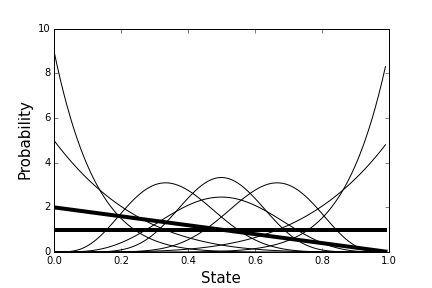
\includegraphics[width=.75\textwidth]{beta-distribution.png}
\caption{Beta distribution for various parameter values of $\alpha$ and $\beta$, including the uniform distribution $\mathcal{B}(1,1)$, and the empirical distribution $\mathcal{B}(1,2)$.}
\label{beta-distribution}
\end{figure}


We use the historical data  in Table \ref{activation-table} from \citet[12]{wallage2013} that shows the number of propositions by activation  to estimate the estimate the prior distribution over states. The degree of activation in these examples is estimated using translations of the texts. However, there are reasons to be confident that activation can reliably be identified in historical corpora.  These figures agree with similar estimates from contemporary corpora. For example, in a sample from a corpus of British English, \cite{tottie:1991} finds that negation is only used 14\% of the time with directly activated propositions. Likewise, in a corpus of American English, \cite{thompson1998} finds that negation is only used 5\% of the time with directly activated propositions. These results suggest that the prior distribution is stable, with the preponderance of negation being used with brand new non-activated propositions. Intuitively, this distribution makes perfect sense: the majority of conversation is about introducing new information rather than treading the same old ground of what has already been said. If the prior distribution is indeed stable, then we can estimate it from the data pooled across time periods. A good fit to the data is the prior probability distribution $\mathcal{B}(1,2)$, also shown in Figure \ref{beta-distribution}.\footnote{We treat each of the discrete categories as equal portions of the unit interval and find values of $\alpha$ and $\beta$ such that $\int_0^\frac{1}{3} \mathcal{B}(\alpha, \beta)(t) dt \approx p(\textsc{non-activated})$, $\int_\frac{1}{3}^\frac{2}{3} \mathcal{B}(\alpha, \beta)(t) dt \approx p(\textsc{indirectly activated})$, and $\int_\frac{2}{3}^1 \mathcal{B}(\alpha, \beta)(t) dt \approx p(\textsc{directly activated})$, where the probabilities are estimated from the totals in Table \ref{activation-table}. Obtaining a better empirical estimate of the prior from contemporary data and intuitions is something we leave for future research.}




\begin{table}
\begin{tabular}{@{}cccc@{}}
\hline
    \textsc{period}   &\textsc{non-activated} & \textsc{indirectly activated} & \textsc{directly activated} \\
\hline
1150-1250    & 393  & 203 & 52   \\
1250-1350    & 346  & 296 & 42 \\
1350-1420    & 294  & 179 & 60 \\ \hline
\textsc{total} &1033 & 678 & 154  \\
\end{tabular}
\caption{Distribution of sentence activation in PPCME \citep{ppcme2} from \cite{wallage2013}}
\label{activation-table}
\end{table}
%We have two functions that we want to maximize with respect to three variables. To do so, we need to find the conditions where the following hold.
%
%\begin{equation}
%	\frac{\partial E[U_S(s, r)]}{\partial t_1^*} = 0
%\end{equation}
%
%\begin{equation}
%	\frac{\partial E[U_R(s, r)]}{\partial a_1^*} = \frac{\partial E[U_R(s, r)]}{\partial a_2^*} = 0
%\end{equation}

To calculate the maxima of the expected utility functions, let $\langle s^*, r^* \rangle$ be an equilibrium strategy profile. In this case, the speaker strategy is defined by $s^*((0, t_1^*)) = \textcolor{red}{m_1}$ and $s^*((t_1^*, 1)) = \textcolor{blue}{m_2}$. Likewise, the hearer strategy is defined by $r^*(\textcolor{red}{m_1}) = \textcolor{red}{a_1^*}$ and $r^*(\textcolor{blue}{m_2}) = \textcolor{blue}{a_2^*}$.  We can determine the evolutionarily stable strategies by jointly maximizing speaker and hearer expected utility. That is, we solve a system of partial differential equations for $t_1^*$, $\textcolor{red}{a_1^*}$ and $\textcolor{blue}{a_2^*}$. For any amount of bias, the maximizing values are shown in Figure \ref{sol2-beta}.\footnote{See Appendix A for the full calculations of the solution.} Along the horizontal axis is the amount of speaker bias, the vertical axis represents the point at which speakers partition the state space and the actions of hearers in response to the forms. For any value of the speaker bias $b$, the solid black line represents the point at which speakers partition the state space $t_1^*$ and the dashed lines represent hearer responses to the different messages, $\textcolor{red}{a_1^*}$ and $\textcolor{blue}{a_2^*}$.

\begin{figure}
	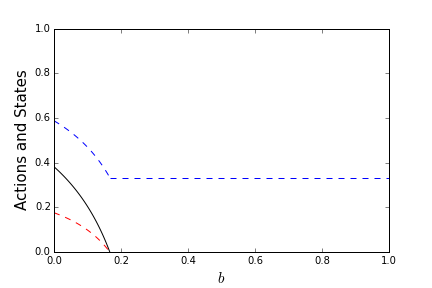
\includegraphics[width=.75\textwidth]{sol2-beta.png}
	%
	\caption{Equilibrium solution for two messages for values of bias}
	\label{sol2-beta}
\end{figure}

So, for example, where $b=.1$ speakers will partition the states at $t_1^*=$, sending $\textcolor{blue}{m_2}$ for all states above this point and sending $\textcolor{red}{m_1}$ for all states above. In response to these forms, hearers will take the actions indicate by the dashed lines, $\textcolor{red}{a_1^*} = $ and $\textcolor{blue}{a_2^*} = $. In fact, these actions correspond to the expected value of the state given the message. That is, $\textcolor{red}{a_1^*} = E[t \mid t < t_1^*]$ and $\textcolor{blue}{a_2^*} = E[t \mid t > t_1^*]$. They are the \emph{Bayes estimators} of their respective signals, the values that maximize hearers' expected utility given a signal.


We are now in a position to answer our first question regarding the relationship between speaker bias and the use of different forms at equilibrium. Namely, if speakers are too biased when it comes to keeping track of common versus private knowledge then only a single message can be used in equilibrium. For example, we can read off of Figure \ref{sol2-beta} that if $b > \frac{1}{6}$ then only $\textcolor{blue}{m_2}$ will be used in equilibrium.\footnote{In fact, for any number of messages $n$ there exists a maximum amount of bias $b_n$ such that all messages are used in equilibrium. For any number of messages \cite{crawford-sobel:1982} show that $b_n > b_{n+1}$. That is, for a given number of messages, there is a maximum amount of bias that allows for all messages to be used in equilibrium. As speakers' bias decreases, $b \rightarrow 0$, the number of messages that can be used in equilibrium goes to infinity. The closer the incentives of senders and receivers, the finer and more detailed the information senders want to signal. The number of messages available is the only limit on the amount of information conveyed when the interests of both parties are perfectly aligned.} When speaker bias is sufficiently large this form carries no information about the activation of the proposition being negated. The \emph{information gain}, or Kullback-Leibler divergence, from receiving the message is zero exactly when the message fails to shift the hearer's beliefs from the prior probability.

\begin{equation}
     KL( \textcolor{blue}{m_2}) = \int_0^1log\left( \frac{p(t \mid \textcolor{blue}{m_2})}{p(t)}  \right)p(t \mid  \textcolor{blue}{m_2}) dt
\end{equation}
If the posterior $p(t \mid \textcolor{blue}{m_2})$ is the same as the prior $p(t)$, as is necessarily the case when a single message is used, then the information gained is zero. This follows directly from the definition of information gain, the logarithm of one is zero. This offers a precise definition of bleaching as the loss of information as a signal spreads across states. 

%Note that this does not mean that \emph{\textcolor{blue}{ne...not}} ceases to carry information as it becomes the only form. Rather, it ceases to carry any information about the activation of the proposition it is being used to negate. 
%An interesting consequence is that the incumbent form becomes more informative as it gets pushed into negating non-activated propositions.
%There are several things to note about the equilibrium solutions for two messages. First, the point at which senders partition the state space strictly decreases in the amount of bias. The more biased that senders are the more that senders will use message $m_2$. For $ b > \frac{1}{6}$ this is the only message that gets used in equilibrium, which is exactly what we see in Figure \ref{sol2-beta}. 
%Second, the receiver's best response to the different messages is the action that corresponds to the expected value of the portion of the partition that it corresponds to. That is, $a_1^* = E[t \mid t < t_1^*]$ and $a_2^* = E[t \mid t > t_1^*]$. These receiver responses are \emph{Bayes estimators}, the actions which maximize the utility function given the receipt of a signal. 

There are two important implications for the functional cycle. First, if speakers are sufficiently biased towards their own perspective when estimating the degree of activation for a proposition, then only a single form is stable. In particular, \emph{\textcolor{red}{ne}} and \emph{\textcolor{blue}{ne...not}} cannot coexist, in fact, only \emph{\textcolor{blue}{ne...not}} can be used in equilibrium. This leads to our second question. Where speaker bias is sufficiently large, are equilibria where only a single form is used evolutionarily stable? In fact, we can show that a signaling equilibria is evolutionarily stable only if all available signals are used. 

To see why this is the case, suppose that the amount of bias only allows for a single form to be used in equilibrium, call it $\textcolor{red}{m_1}$. Now, suppose further that there is an additional form that is not used in equilibrium, $\textcolor{blue}{m_2}$. The action that hearers would take in response to this unused message can vary without affecting the expected utility of speakers or hearers. This means that the equilibrium is not strict, and therefore is not evolutionarily stable.  In particular, a single-form equilibrium can be disturbed by the introduction of a new message, it is not \emph{neologism-proof} \citep{farrell:1993}. For example, suppose that a new form is only used for high degrees of activation, and that hearers respond by inferring a high degree of activation. Given speakers' bias, there will be additional states that speakers think warrant using the new form. In response to this increase, hearers will infer a lower degree of activation, meaning additional states will be used by speakers, and so on. This holds for any pair of messages $m_i$ and $m_{i+1}$. 

Importantly, this is just the functional cycle as we have been describing it.  So, even though two forms may not be stable for a sufficiently large degree of speaker bias, a single form is never evolutionarily stable. The functional cycle can always be set in motion by the introduction of the appropriately conditioned form. This means that just as \emph{\textcolor{red}{ne}} can be pushed out by \emph{\textcolor{blue}{ne...not}}, so too could \emph{\textcolor{blue}{ne...not}} be pushed out with the introduction of the right new form, one that is initially restricted to high degrees of activation.

%Note that this is just a description of the functional cycle. We could abstract over indices and note the same thing about any two signals $m_i$ and $m_{i+1}$.


%	\item This gives a general flavor for the dynamics
%	\item But, we need explicit evolutionary game dynamic
%\end{itemize}

\section{Dynamics}

While we can reason about how speakers and hearers might react to the introduction of a new form, this kind of equilibrium reasoning is essentially static. That is, it allows us to reason about what would happen if we started at a particular state, but not whether we will ever reach that state in the first place. More importantly, it does not allow us to examine how a population evolves from any starting state in general. To understand how speakers and hearers change over time, we must posit a process that underlies how speakers and hearers interact and respond to each other. Doing so will allow us to examine how different degrees of speaker bias impact the trajectory of meaning. First, we discuss the replicator dynamics as an appropriate evolutionary game dynamics for studying changes in meaning.  Then, we simulate trajectories of a population interacting over time. 

%Second, we define the necessary components for the replicator dynamics of the game described in the previous section.

The replicator dynamics were originally introduced as an explicitly dynamic model of biological replication, but have since been shown to have deep connections with some of the most widely-studied models of learning. In particular, \cite{borgers-sarin1997} prove that the expected behavior of agents playing an asymmetric game while learning according to a \emph{linear reward-inaction} scheme \citep{bush-mosteller1955} is equivalent to the asymmetric replicator dynamics if the agents interact frequently and change their behavior slowly. That is, if individuals tend to do things that are more successful, then their expected behavior can be modeled by the replicator dynamics.

If we assume that speakers and hearers learn in this manner, there are a few conceptual clarifications to be made to justify the use of the replicator dynamics in modeling the functional cycle. First, we need to be sure that speakers and hearers interact frequently and change their behavior slowly. Both of these would seem to follow from the overall frequency of negation. Given that negation is one of the most frequently used forms in any language, it is safe to assume that speakers and hearers  interact frequently and do not dramatically alter their use or interpretation of negation from one sentence to the next.  Second, we assume that each individual acts as a speaker and hearer, but cannot introspectively reason about the impact of one on the other. That is, individuals cannot use their behavior as speakers to change their own behavior as hearers, nor vice versa. Third, while the replicator dynamics can be used as a model of individual learning, we are interested in how the population as a whole changes. However, given that the \emph{expected} behavior of individuals is equivalent to the replicator dynamics under this kind of learning, then the expected behavior of a population of individuals should be as well. That is, if averaging at the individual level yields the replicator dynamics, then so should averaging over averages.  This is akin to treating the populations of speakers and hearers \emph{as if} they were individuals. 


We simulate the change in the proportion of the different forms over time for a population evolving according to the replicator dynamics from the same starting conditions.\footnote{Here we use the discrete-time replicator dynamics for computational tractability, whereas the results presented by \cite{borgers-sarin1997} hold for the continuous-time replicator dynamics. While the two dynamics are substantially similar for our purposes, we leave a comparison for future work. Note that we also discretize the set of states and actions for speakers and hearers, respectively. That is, for some $n$, we treat the set of states $T : \{t_0, ..., t_n \}$ and actions $A : \{a_o, ..., a_n \}$, where $t_i = a_i = \frac{i}{n}$. See Appendix B for full details of the numerical simulations.}  In this case, the population starts off from a state where speakers only use \emph{\textcolor{blue}{$m_2$}} for high degrees of activation and hearers respond by inferring a high degree of activation. Varying the bias parameter $b$ yields the trajectories shown in Figure \ref{rd-multiple}. Along the horizontal axis we have time, and along the vertical axis we have the proportion of \emph{\textcolor{blue}{$m_2$}} used at any point in time. For sufficiently large amounts of speaker bias, the incoming form is guaranteed to replace the incumbent form, the amount of bias controls the rate at which this happens.  For sufficiently small amounts of speaker bias, both forms are guaranteed to persist.


\begin{figure}
\centering
     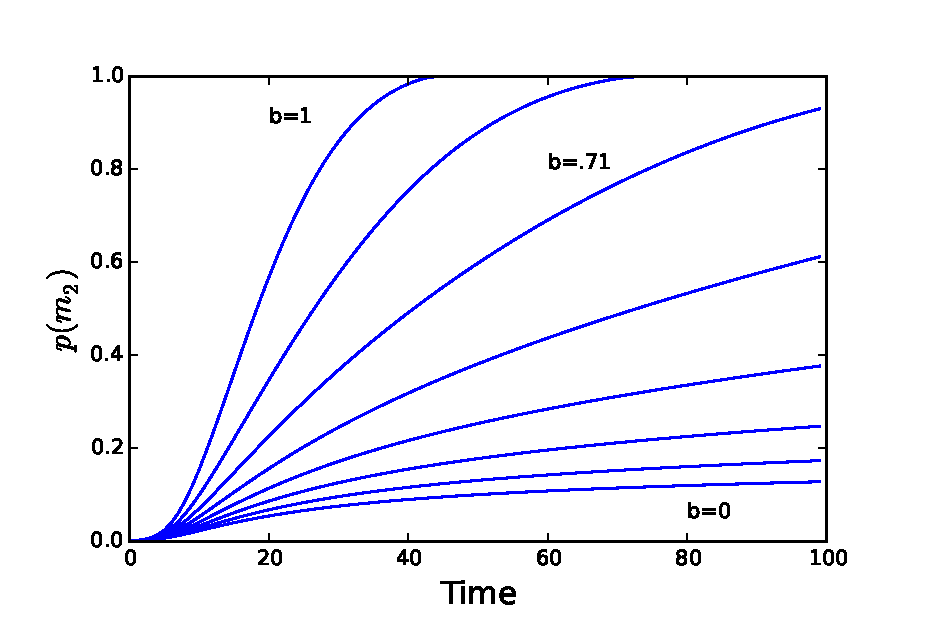
\includegraphics[width=.75\textwidth]{replicator-multiple-b.eps}
\caption{Proportion of $m_2$ under the discrete-time replicator dynamics for varying amounts of speaker bias}
\label{rd-multiple}
\end{figure}

So, our numerical simulations agree with the predictions from the static equilibrium analysis. If speaker bias is too large, then only a single form is used. More specifically, the form that is used at equilibrium is the form that started off restricted to higher degrees of activation. Now, while these simulations yield qualitative information about the dynamics of the functional cycle, we are interested in how this model can be used to understand the details of the functional cycle in the history of English. We now turn to fitting the model to historical trajectory of negation in English.


\section{Modeling}

Defining the stage game and the evolutionary dynamics allowed us to investigate the effect of speaker bias on the functional cycle in the abstract, but we are really interested in how the resulting model can be used to explain the actual historical trajectory of negation in a concrete case. In particular, we are interested in what happens when we fit the model to data from the history of negation in English. First, we describe the data that we fit the model to. Second, we define the parameters of the dynamics that we fit. Finally, we evaluate these parameters in light of the experimental data presented above.

The data we use are drawn from the PPCME2 \citep{ppcme2}. All tokens used are negative declaratives, excluding cases of contracted negation as well as cases that appear to be constituent negation.\footnote{We model the data used here after \cite{wallage2008}, which makes a compelling argument for treating contracted negation, among other cases, separately. Many thanks go to Aaron Ecay for sharing the code for generating the queries.} Each circle represents tokens in a given year. The size of the circle represents the number of tokens. The height of the circle represents the proportion of those instances that are a particular form. Locally-weighted regression lines are fit to these proportions. We see the transition from \textit{\color{red} ne} to \textit{\color{blue} ne...not} starting around the 12th century, followed closely by the transition from \textit{\color{blue} ne...not} to \textit{\color{green} not} in the 14th century.

\begin{figure}
\centering
     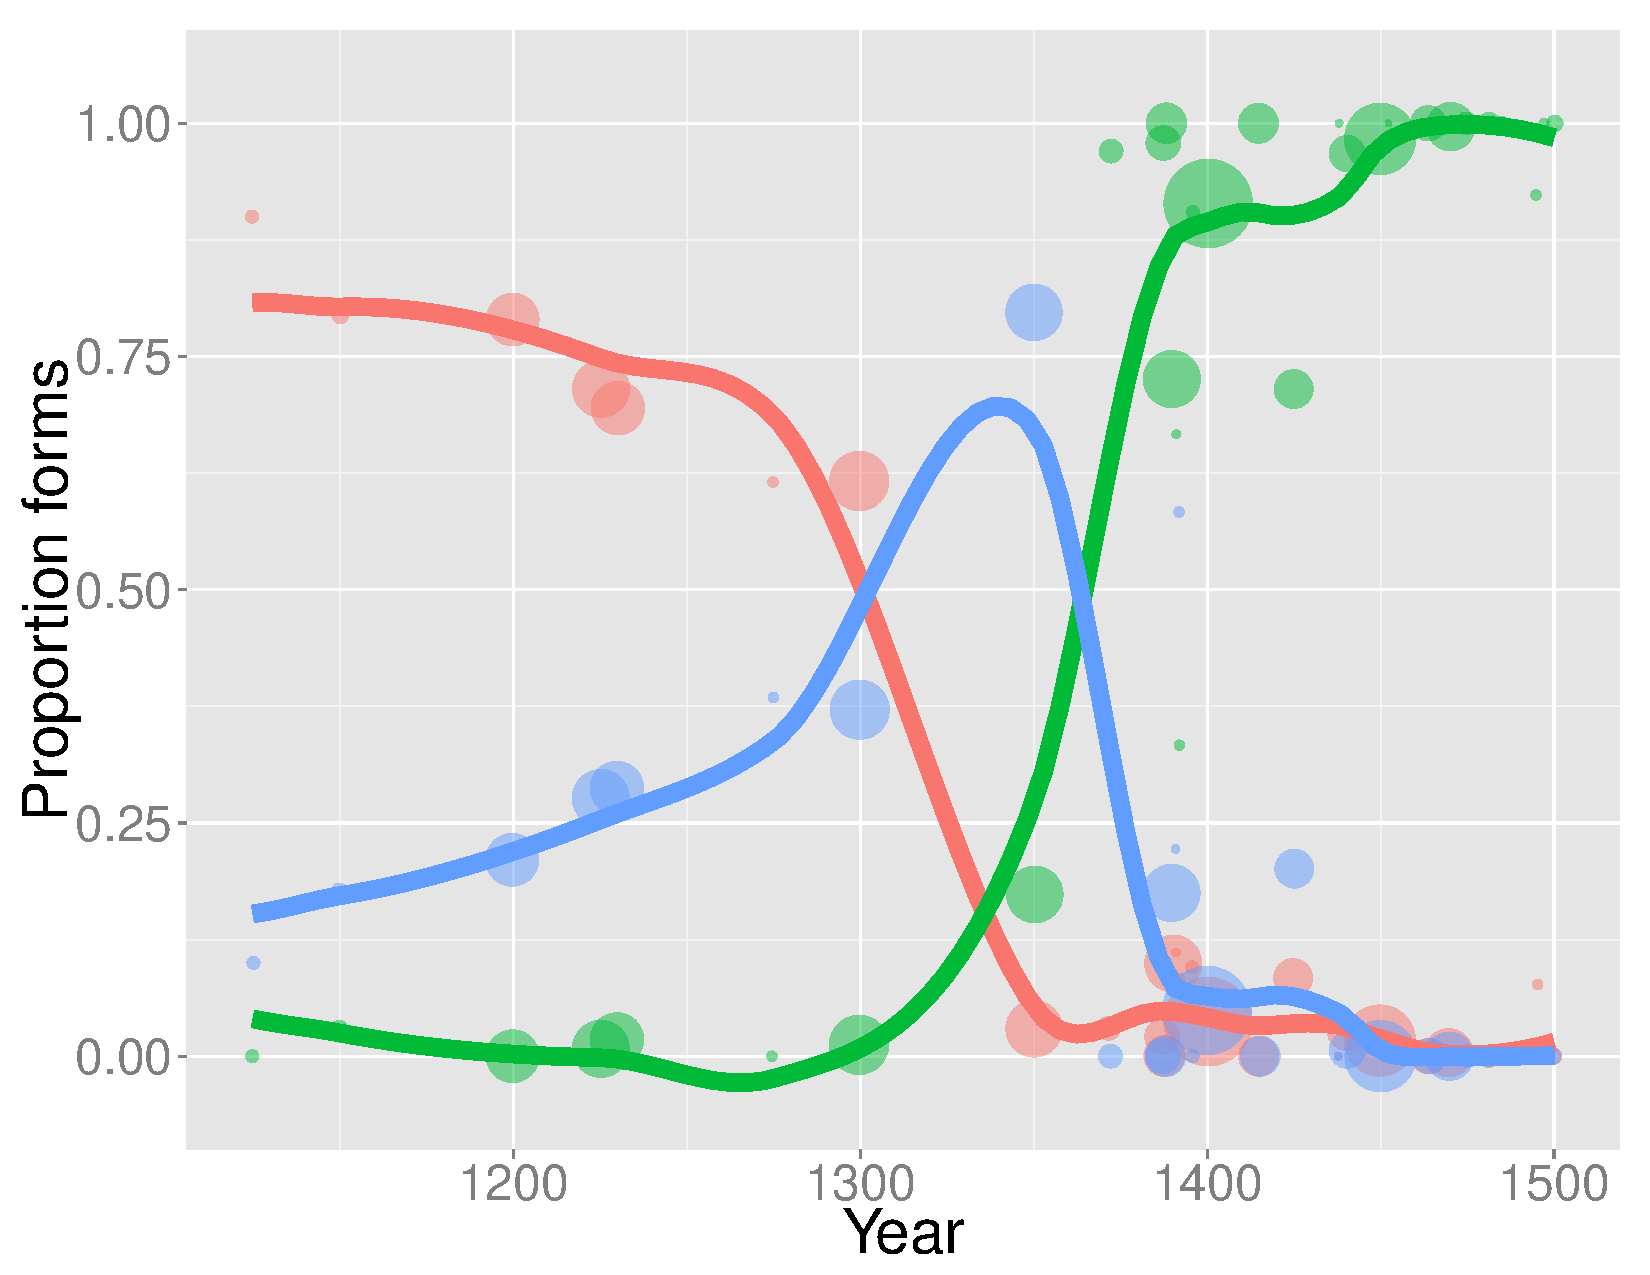
\includegraphics[width=.75\textwidth]{neg-year-lines.pdf}
\caption{Proportion of \textit{\color{red} ne}, \textit{\color{blue} ne...not}, and \textit{\color{green} not}  in Negative Declaratives}
\label{neg-three-plot}
\end{figure}

Now, given that we are interested in the functional cycle, we care about the transition from \textit{\color{red} ne} to \textit{\color{blue} ne...not}. That is, we care about an incoming emphatic form displacing an incumbent form. So, the subsequent rise of \textit{\color{green} not} is the second transition in the formal cycle, but not a part of the functional cycle. How should we deal with \textit{\color{green} not} in our analysis? There are two possibilities. First, we could ignore \textit{\color{green} not} and simply fit the model to the proportions of \textit{\color{red} ne} and \textit{\color{blue} ne...not}. The problem with doing so is that this attributes too much to small fluctuations in the proportions of \textit{\color{red} ne} and \textit{\color{blue} ne...not} even if those fluctuations are not meaningful in any sense relevant to the model. It is unlikely that small changes in the 15th century are something that we want to model.

Second, we could ignore the distinction between \textit{\color{blue} ne...not} and \textit{\color{green} not}, and treat them as if they were the same form. This alleviates the potential problem of attributing too much meaning to small fluctuations past a certain date. More importantly, it captures the contingency of the second transition of the formal cycle to purely post-verbal negation. That is, the rise of \textit{\color{green} not} is not a part of the functional cycle, nor is it a necessary and immediate consequence of the functional cycle. We only need to compare the history of negation in French where the embracing form goes to completion before being eventually replaced by the post-verbal form. Taking this route allows us apply the same model across languages without regard to subsequent contingent developments. The results of doing so are shown in Figure \ref{lump-plot1}.


\begin{figure}
\centering
     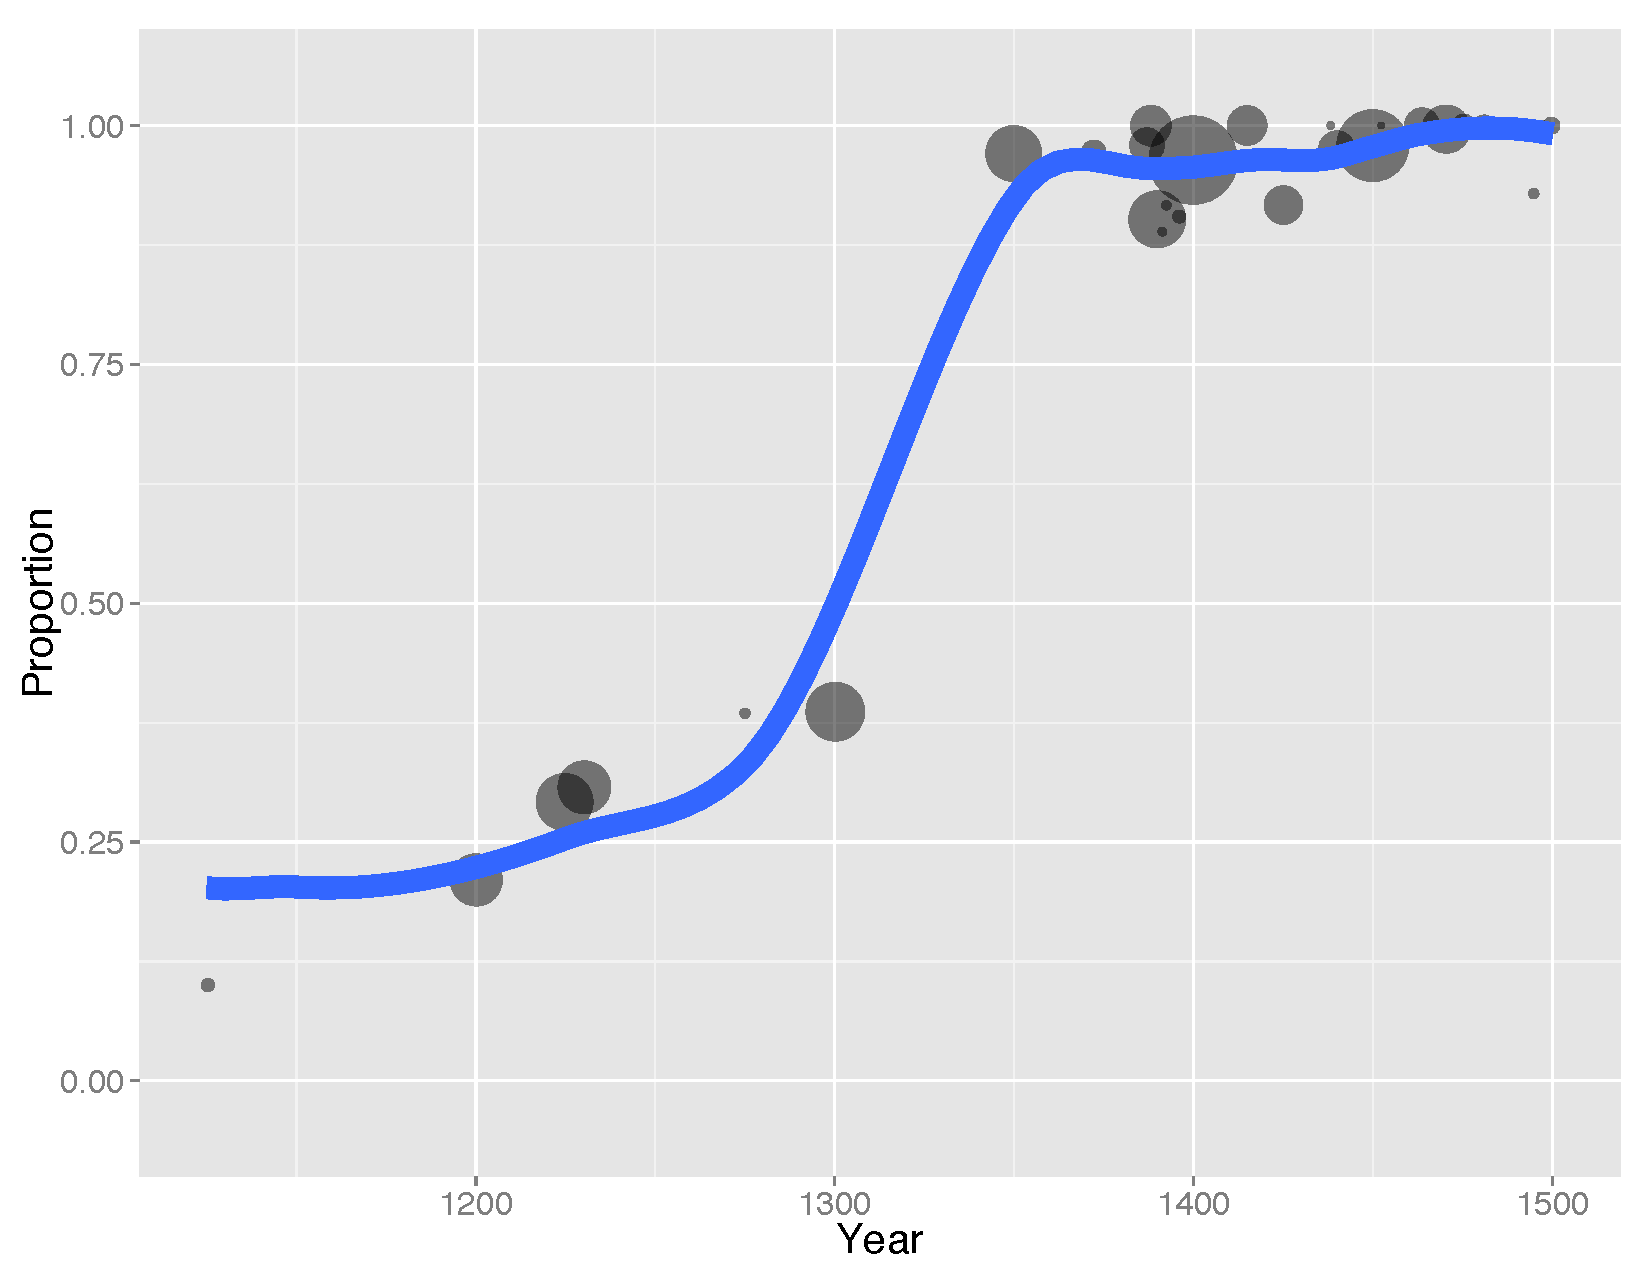
\includegraphics[width=.75\textwidth]{lump-plot1.pdf}
\caption{Proportion of \textit{\color{blue} ne...not} and \textit{\color{green} not}  versus  \textit{\color{red}  ne} over time}
\label{lump-plot1}
\end{figure}

Taking the trajectory of forms in Figure \ref{lump-plot1} as the data we want to fit our model to, we need to specify the parameters of the model to be fit. In particular, we need to define the initial state of how speakers use the different forms and how hearers respond to them. In fact, we have quite a bit of information regarding what the initial state of the functional cycle actually is. That is, we know that \textit{\color{blue} ne...not}   is fairly infrequent and largely restricted to high degrees of activation. Likewise, we know that hearers' response to \textit{\color{blue} ne...not}  is also largely restricted to actions corresponding to high degrees of activation. We can translate this information into conditions on the initial states of the speaker and hearer populations.

Regarding speakers we assume that both forms have a particular meaning, which is captured by conditional probability of states given a form. Namely, \textit{\color{red} ne} is the default form and does not carry any information above and beyond the prior, it roughly satisfies the following conditional distribution $p(t \mid \textcolor{red}{ne}) \sim \mathcal{B}(1, 2)$. In contrast, \textit{\color{blue} ne...not} is overwhelmingly used in states with high degrees of activation, that it satisfies the following conditional distribution $p(t \mid \textcolor{blue}{ne...not}) \sim \mathcal{B}(\alpha, 1)$. The larger $\alpha$ is, the more skewed towards high degrees of activation is \textit{\color{blue} ne...not}. Note that these two distributions along with the prior determine the initial proportion of \emph{\textcolor{blue}{ne...not}}. So, we only have a single parameter $\alpha$ to fit for the initial state of speakers.

%Moreover, if the initial proportion of the incoming form is sufficiently small then the incumbent form necessarily approximates the prior distribution.

Regarding hearers, we assume that the expected value of the responses to both forms correspond to the expected value of the conditional probability of states given the form. Intuitively, this corresponds to hearers starting off with a fairly accurate responses to the two forms. For \textit{\color{red} ne} this is satisfied by any distribution $\mathcal{B}(\alpha, \beta)$ such that $\alpha = \frac{1}{2}\beta$, which has an expected value $\frac{\frac{1}{2}\beta}{\frac{1}{2}\beta + \beta} = \frac{1}{3}$. Note that is the same as the expected value of the conditional probability of the state given the message $p(t \mid \textcolor{red}{ne}) \sim \mathcal{B}(1, 2)$.  So we take the conditional probability of actions given \textit{\color{red} ne}   to be $p(a \mid \textcolor{red}{ne}) \sim \mathcal{B}(\frac{1}{2}\beta_1, \beta_1)$. All that $\beta_1$ does is to determine how concentrated the action is around the expected value.  For \emph{\textcolor{blue}{ne...not}} let $\gamma = E[t \mid \textcolor{blue}{ne...not}]$, then this is satisfied by any distribution $\mathcal{B}(\alpha, \beta)$ such that $\alpha = \left( \frac{\gamma}{1 - \gamma} \right)\beta$, so we take the conditional probability of an action to be $p(a \mid \textcolor{blue}{ne...not}) \sim \mathcal{B}(\left( \frac{\gamma}{1 - \gamma} \right)\beta_2, \beta_2)$.  Again $\beta_2$ determines how concentrated the action is around the expected value. So, we have two parameters $\beta_1$ and $\beta_2$ to fit for the initial state of hearers.

The last thing to note before fitting the model is the notion of time. That is, the replicator dynamics specify how populations change from one point in time to the next, but how these abstract units correspond to days or years is unspecified. In what follows we treat each of these abstract time units as a year, but leave open the possibility that another proportion may be more appropriate. One option would be to treat the ratio between years and abstract time units as another parameter to be fit in the model, but for now we leave this as an avenue for future research.

We fit the initial state parameters and bias parameter to the data.\footnote{See Appendix B for the full details of the starting states and the resulting fit.} We begin by visualizing the overall trajectory of the incoming form, then turn to the change in the meaning of the two forms over time.  Figure \ref{m2-sol} shows the predicted proportion of \textit{\color{blue} ne...not} over historical time for the fitted model with the bias parameter $\hat{b} = 0.49132877$. Perhaps more importantly, we can actually inspect the inner workings of the model as they relate to the functional cycle.

\begin{figure}
\centering
     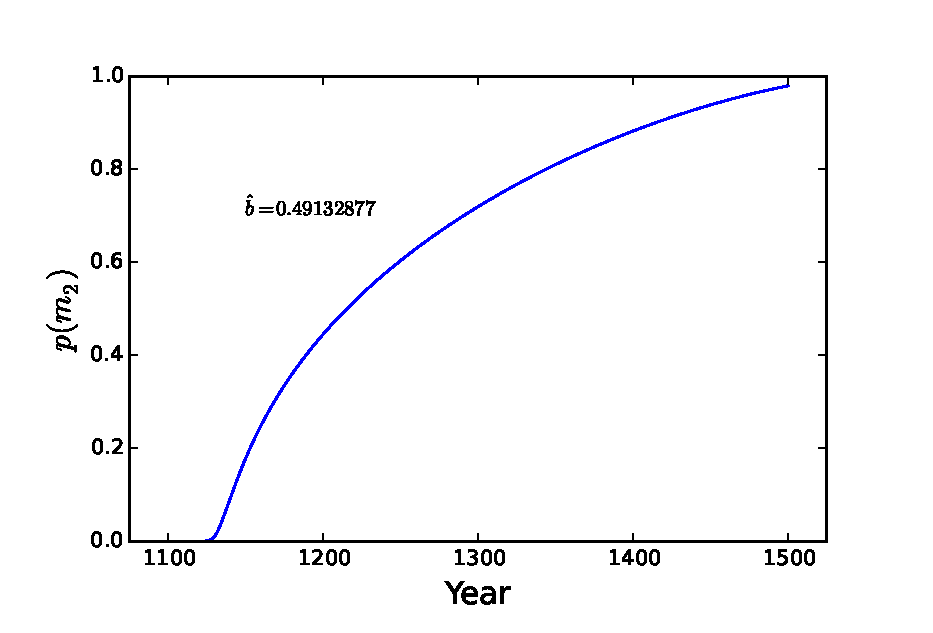
\includegraphics[width=.75\textwidth]{m2_sol.eps}
\caption{Predicted probability of \textit{\color{blue} ne...not} over time for fitted model of functional cycle.}
\label{m2-sol}
\end{figure}

In particular, we can examine how the information carried by the two forms changes over time. We gain insight into the functional cycle by considering how the meaning of \emph{\textcolor{blue}{ne...not}} changes over time as in Figure \ref{m2-meaning}. The horizontal axis represents states and vertical axis represents the conditional probability of states given that \emph{\textcolor{blue}{ne...not}} was used. We show this conditional probability at various points as the functional cycle proceeds. The dashed line indicates the prior probability distribution over states. The initial meaning of the incoming emphatic form is represented by the curve with the most rightwards skew. This indicates the point at which the incoming emphatic form carries the most information and is thus the most emphatic.  But, as time goes on, \emph{\textcolor{blue}{ne...not}} spreads to more and more degrees of activation as it the form increases in frequency. We represent this with subsequent distributions that move more and more towards the prior distribution. As they do so, the form loses its emphasis, as indicated by the thickness of the line. When \emph{\textcolor{blue}{ne...not}} is the only form, it carries no information about activation beyond the prior. Visually speaking, at this point its emphasis has faded entirely.


\begin{figure}
\centering
     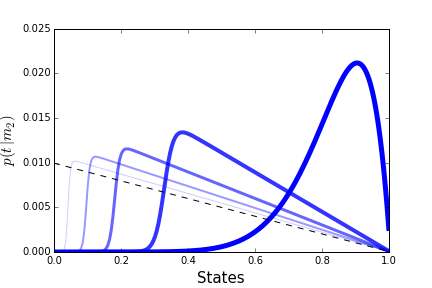
\includegraphics[width=.75\textwidth]{p_t_m2_rd.png}
\caption{The emphatic form over time as given by the conditional probability of states given \textit{\color{blue} ne...not}, where dashed line indicates prior probability distribution.}
\label{m2-meaning}
\end{figure}

We also gain insight in to the functional cycle by comparing the relative meaning of both forms. Comparing the meaning of \emph{\textcolor{red}{ne}} at the outset of the cycle and \emph{\textcolor{blue}{ne...not}} at the end of the cycle is particularly informative. Figure \ref{push-chain} emphatically demonstrates the dynamics of the push-chain scenario. At the beginning of the cycle in 1125 CE,  \emph{\textcolor{red}{ne}} carries no information about the degree of activation, it coincides with the prior as indicated by the dashed line.  In contrast, \emph{\textcolor{blue}{ne...not}} is overwhelmingly restricted to cases where the proposition being negated has a high degree of activation. Both of these facts are shown in the top panel of Figure \ref{push-chain}. But, one hundred years later, \emph{\textcolor{blue}{ne...not}} has expanded to more states as it increases in frequency and \emph{\textcolor{red}{ne}} is pushed to lower and lower degrees of activation. This is shown in the second panel of Figure \ref{push-chain}. As the functional cycle proceeds, the old form is pushed lower and lower down the scale. Eventually, the incoming form has displaced the incumbent form and ceases to carry any information about the degree of activation.

\begin{figure}
\centering
     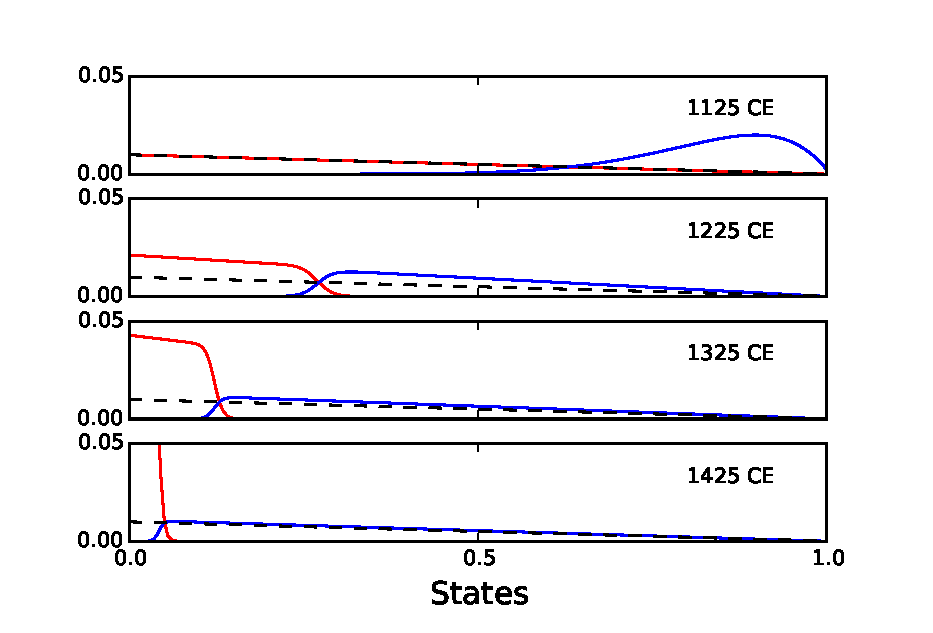
\includegraphics[width=\textwidth]{push_chain.eps}
\caption{The push-chain of the functional cycle given by the conditional probability of states given form at various points in time, where dashed line indicates prior probability.}
\label{push-chain}
\end{figure}

So, the dynamics of the fitted model match our theoretical conceptions of the functional cycle as a kind of push chain. The incoming form pushes the incumbent form out, eventually taking its place and losing its emphasis. Given that the driving force behind this change was posited to be speakers' bias to overestimate activation, it is important to take a moment to evaluate the value of the fitted bias parameter, $\hat{b}$. Given that the incoming form replaces the incumbent form, we would expect from our equilibrium analysis that at the very least $\hat{b} > \frac{1}{6}$, but this still leaves a fair amount of room for the parameter to vary. In fact the fitted value $\hat{b}=.4913287$ is well above this minimum. 

Now, given this value, we might ask whether it is reasonable in light of the experimental results discussed above. To evaluate the parameter, we return to the results reported in \cite{wu-keysar2007}. Namely, when playing a communication game, speakers relied on private knowledge of the names of shapes in a proportion of trials. We can use this information to estimate the expected value of the bias parameter exhibited by speakers in the experiment. 

To see this, first suppose that there are only two states corresponding to whether or not the name for a particular shape was learned privately or jointly. That is, knowing whether a name was learned privately or jointly is categorical. As \cite{heller-etal2012} found, this is a reasonable assumption given that participants were incredibly accurate at recalling the context of learning for shapes. Second, suppose that the utility functions for both speakers and hearers are the same form as above. Third, suppose that hearers take one action in response to names and another for descriptions that correspond to initial guesses about the status of the target shape. Then a speaker would only prefer the action taken in response to a name for a privately learned shape if $b > \frac{1}{2}$. 

But, this preferences is not categorical. In fact, from the experimental results we only know the probability that $b > \frac{1}{2}$. However, we can estimate the expected value of the bias parameter. Let $p(b) \sim \mathcal{B}(\alpha, \beta)$ be a distribution over the unit interval. We find the parameters such that $\int_\frac{1}{2}^1 p(b)db = p(b > \frac{1}{2})$, which in turn give the expected value of $b$. For example, where speakers use a privately known name in 5\% of trials $E[b] = .1398$, and where speakers use a privately known name in 28\% of trials $E[b] = .3549$.  

So, there are a range of potential values of speaker bias that we can estimate from the experimental evidence. In both cases these are smaller than the fitted value of the bias parameter for the functional cycle. However, there are good reasons to treat these experimental estimates as lower bounds. First, the fitted parameters deal with different domains. Where the experiments deal with the referential domain, the functional cycle deals with the propositional domain. It is certainly possible that speaker bias varies across these domains. In fact, we might even expect this. For example, referents often come along with some externally observable entity in the real world, whereas propositions often do not. The fact that propositions are in this sense more abstract may lead speakers to rely on their own perspective more.  Second, the experiments found speaker bias even between strangers. These kinds of communicative biases are even more pronounced between people who know each other well \citep{savitsky-etal:2011}.\footnote{For example, one day when I got home the first thing my wife said to me was, ``I \textsc{did} make an appointment.'' This struck me as out of the blue, but she said that she told me that she was feeling a little under the weather and debating whether her cold symptoms warranted a trip to the doctor. This conversation had happened several days prior and I had completely forgotten about it, but it was on her mind. In other words, her own subjective estimate of $p =$``I made a doctor's appointment.'' was greater than the actual degree of activation. In this case, I would say that the bias was fairly high $b \approx 1$.} Thus the degree of speaker bias in everyday life may be significantly larger than these experimental estimates suggest.

Careful experimentation will be needed to nail down how private and common knowledge are tracked in the propositional domain, and how this plays out in everyday life. However, the results are largely compatible with both the mechanics of the dynamic model of the functional cycle we have defined here.

\section*{Summary}

Separating out the formal and functional cycles lightens the explanatory burden. By isolating the functional cycle we were able to identify what conditions the incoming form and reason about why those conditioning factors change over time. In particular, we argued that speakers have difficulty in keeping track of private versus common knowledge, which biases them towards overestimating the activation of propositions being negated. The tools used to model the functional cycle allow us to offer the first explanatory model of the dynamics of how meaning changes over time.  Importantly, they also highlight the fact that while the driving force of the functional cycle is a byproduct of our cognitive limitations in tracking common knowledge, change comes about through the social interactions between individuals in a population.  Thus explaining the functional cycle requires a model of how pragmatic competence shapes signaling over time.

Before moving on, we pause to consider two potential lines of research related to the model we have discussed here. The first deals with the alternative definition of emphasis offered at the outset. That is, emphatic negation widens and strengthens negation to preclude exceptions. This interpretation is appealing insofar as negative polarity items are often recruited to create emphatic forms and have exactly this effect \citep{kadmon-landman1993any, eckardt2006}. However, this approach to the functional cycle would have to do two things. First, it would have to specify what serves the role of speaker bias in driving the increase of an incoming emphatic form. Second, it would have to address the problem of over-prediction. That is, if new signals can be formed with the addition of any negative polarity item, then there will always be new forms available, and thus the functional cycle should always be occurring. The fact that we do not observe Jespersen's treadmill means there must be some kind of restriction on what can serve as a new emphatic form. One potential restriction is that the new form must be free from sortal restrictions. For example, both ``I didn't move a crumb" and ``I didn't eat a crumb" must be equally acceptable.

The other line of research has to do with the implications of this model of the functional cycle for referring expressions that are also sensitive to degrees of activation. \cite{gundel-etal1993} refer to the scale of sensitivity as the \emph{giveness hierarchy}, which is roughly ordered by pronouns, demonstratives, definites, and indefinites. Pronouns are restricted to referring to entities that are directly activated, whereas indefinites can be used with any entity. Interestingly, similar diachronic patterns are observed as forms spread to lower degrees of activation. For example, the Modern English definite \emph{the} comes from the Old English demonstrative \emph{se}.\footnote{I cannot help but note discussions along this line with Jon Stevens (p.c. March 26, 2010):  ``One long term goal of this sort of research could be to connect it up with facts about language learning and pragmatics (perhaps using game theoretic tools) to paint a larger picture of why grammaticalization phenomena are so pervasive across languages.  As I alluded to in my vignette yesterday, a good model of semantic learning will likely interact with pragmatics in an interesting way; if such modeling techniques become sophisticated enough so as to model the acquisition of grammatical forms as well as content forms, then predictions will be made about the actuation and spread of bleaching, which could serve as a nice test of a model's plausibility."} However, there are at least two interesting implications of the model of the functional cycle for the stability within the givenness hierarchy. First, we would predict greater stability in these referential terms given the prior distribution over degrees of activation. If propositions are largely skewed towards being non-activated, then referents are largely skewed towards being activated. This change in the distribution largely counteracts any amount of speaker bias. Second, the generation of new pronouns, demonstratives, or definites is arguably a rare event. At least, it would seem rarer than a form of negation becoming associated with activation. We leave exploring both these lines of research for the future.

%\begin{itemize}
%	\item givenness hierarchy
%	\item In focus, activated, familiar, unique, referential, type
%	\item Old english : demonstrative to definite
%	\item Why does it change less?
%	\item Different prior distribution $\mathcal{B}(2,1)$, different bias
%	\item Less frequent introduction of new signals
%\end{itemize}



% Bibliography
\bibliographystyle{mcbride}
\bibliography{ahern}

\end{document}